\section{Model and Methods}

\begin{center}
\textbf{---Figure \ref{fig.model_outline} about here---}
\end{center}

\begin{figure}
\centering
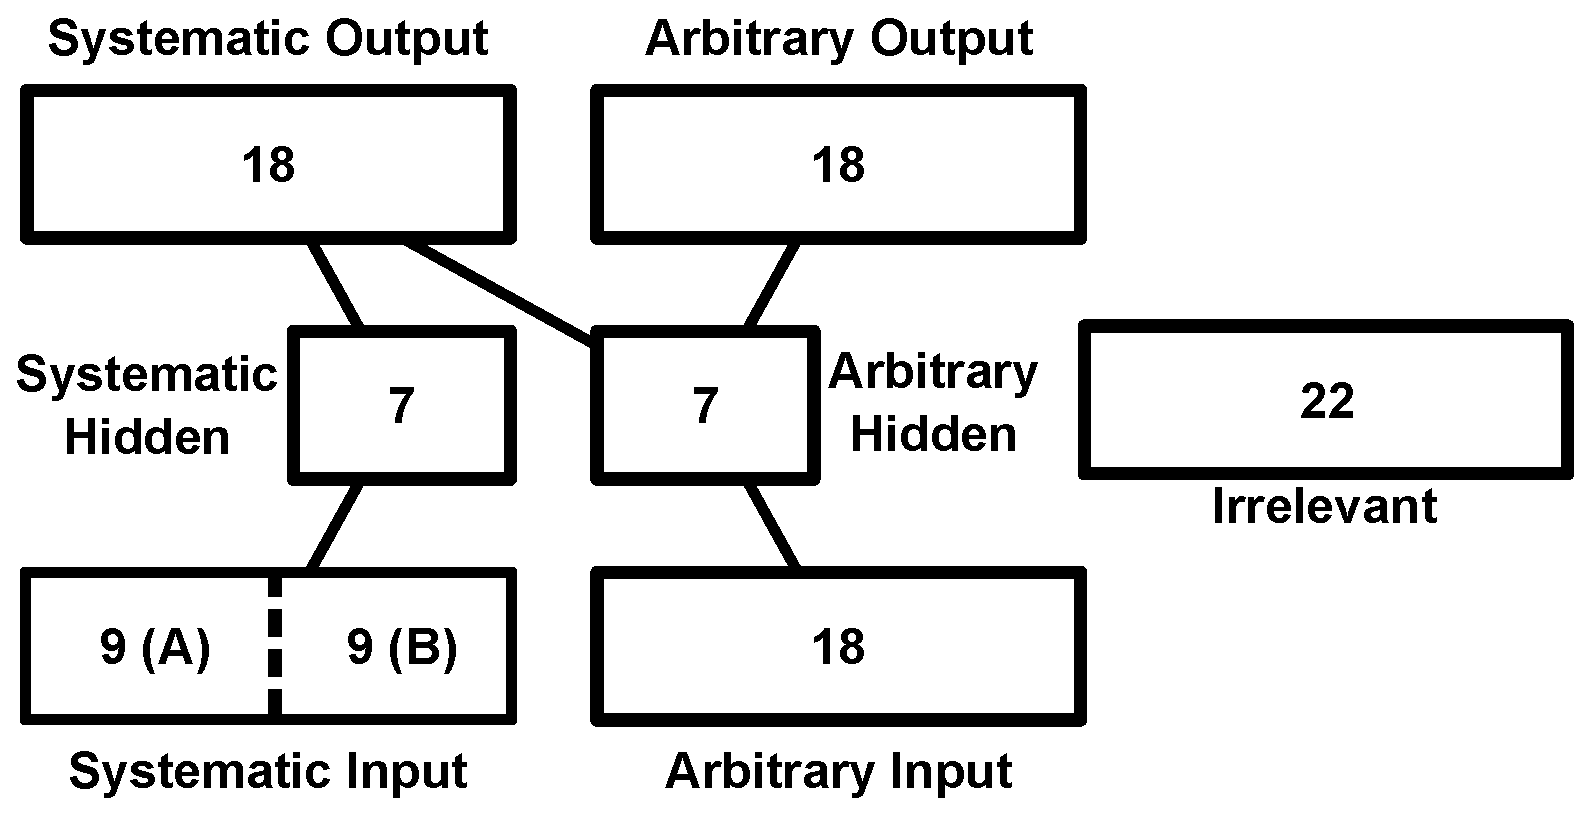
\includegraphics[width=0.75\textwidth]{figures/figure2.eps}
\caption{\label{fig.model_outline} Architecture of the auto-encoder network used to generate the data for 10 model subjects used in subsequent simulations. The model has 36 input units (18 systematic), 14 hidden units (7 systematic), and 36 output units (18 systematic). The 22 irrelevant units are completely disconnected from the network, and stand for units that subserve an unrelated function but are anatomically adjacent to units of interest.}
\end{figure}

The model we will employ for these analyses is illustrated in Figure 2. It is an auto-encoder network: when presented with an experience in the form of a pattern of activity over its 36 input units, it learns to reproduce that same pattern over its 36 output units. Auto-encoder networks have been used as simple models of human memory, because once they have learned they are capable of both retrieving full information from a partial cue and of generalizing prior learning to new items \cite{McClellandRumelhart85}. In this case, however, we do not intend the model to embody a specific hypothesis about a particular real-world cognitive function. Instead, it is designed to make explicit the challenges noted in the introduction. 

To this end, the patterns that the model processes are viewed as coming from two different domains, A and B, corresponding to some cognitive distinction of theoretical import. For instance, A and B might correspond to nouns versus verbs, or animals versus manmade objects, or faces versus non-faces, or any other binary distinction thought to be of potential relevance to behavior. Each individual item is represented with a unique pattern of activation over input units, and the network's task is simply to generate the same pattern over output units. In this sense, there is no explicit representation of the two classes A and B in the inputs, outputs, or network task. The two domains are assumed, however, to be distinguishable from the distribution of input/output properties they possess. Specifically, one subset of input/output properties is marginally more likely to be active for items from domain A, while another subset is marginally more likely to be active for items in domain B. We will refer to these subsets together as {\em systematic I/O} units, because they each weakly covary with the representational distinction of interest.  Each item also possesses several features coded by {\em arbitrary I/O} units whose activations do not systematically differ between domains.

After the model has learned, it is possible to ``query'' it by presenting an input pattern and generating patterns of activation throughout the rest of the network. As noted earlier, we take the activation at each unit in response to an input as a model analog of the neural response to a stimulus estimated from the BOLD signal at a single voxel in a single individual. Across different training runs, the model will always exhibit the same overt behavior (generating the correct pattern over output units), but arising from different configurations of weights, and hence from different internal representations. Variability in weight configurations and internal representations acquired across different training runs thus provides a model analog of individual variability in the neural representations acquired across the population. To simulate data generated by a functional brain imaging study with, say, 10 participants, we train the model 10 times with different random initial weight configurations. For each trained model, we record the pattern of activation generated over all model units by each input pattern (i.e., stimulus), taking these as model fMRI data.  The question we then wish to ask, by applying different statistical methods to the analysis of this synthetic imaging data from a sample of trained models, is the following: which units in the network encode representations of the domains A and B, and how?

The network architecture is designed so that there are two possible answers to this question. The first answer is that representations of A and B are directly encoded in the individual activations of the systematic I/O units. For all input and output units, the response of a given unit to a particular item is directly specified by the environment, so that these units will always respond to a given stimulus in the same way across model individuals. Each systematic I/O unit has a marginally different probability of being active depending upon the domain; in this sense the A units each independently encode a representation of the A domain and the B units encode a representation of the B domain. The relationship between domain and activation is, however, stipulated to be quite loose: for each domain, only a small number of the corresponding systematic units will be active for any given item---each unit participates in just a few patterns. Each item thus overlaps in their systematic properties with just a few other items in the domain, and the correlation between activation and domain is weak for any individual unit.  We further stipulate that the A input and output units are anatomical neighbors, as are the B input and output units, and that this anatomical arrangement is exactly the same across individuals. Thus the systematic I/O units individually encode a {\em weak} distinction between A and B that is {\em consistent} across model individuals and is {\em anatomically localized} within input and output layers.

The second answer is that the representations of A and B domains are encoded in a distributed fashion over a subset of model hidden units. As shown in the Figure, the input units project to the output units by way of two separate hidden layers. The {\em systematic hidden layer} (SH) contains 7 hidden units that receive connections from the systematic input units and send connections to the systematic output units. The {\em arbitrary hidden layer} (AH) also contains 7 units that receive connections from the arbitrary inputs, and send connections to {\em both} the systematic and arbitrary outputs.  The weights are shaped by learning, so every input generates a pattern of activation---a learned internal representation---over both the SH and AH layers. The particular way that layers are connected, however, ensures that these internal representations will have specific representational properties. The SH layer connects systematic inputs to systematic inputs. Because items within a domain have a weak tendency to share systematic properties, the SH units can efficiently perform their mapping by representing the domain structure: items within a domain evoke similar patterns over units and items from different domains evoke quite different patterns. The AH layer receives inputs only from the arbitrary input units and directs outputs to all units. There is no tendency for items within a domain to share arbitrary features, so there is little pressure for these units to represent the domain structure. The AH layer thus acquires distributed internal representations that have little obvious structure. The weights in the arbitrary pathways effectively serve to ``memorize'' both the arbitrary features and the idiosyncratic differences among items in the same domain. In other words, the architecture produces a division of labor in which the SH layer learns distributed representations of the domain structure and the AH layer learns idiosyncratic differences among items. A good method, then, should identify SH units as important for representing the domains.

Indeed, the SH units arguably provide a better encoding of the domain structure than do the systematic I/O units. To illustrate this we first trained the model to saturation on 15 runs with different initial random weights, then analyzed, for each layer in the model, the Euclidean distance between the patterns of activation elicited by each pair of stimuli in the model. For each layer, we computed the mean distances for pairs within a domain and for pairs in different domains. We then took the ratio of between-domain to within-domain distances as a measure of how well the domain structure is expressed in each layer. A ratio of 1 indicates that between- and within-distances are about the same; a number greater than 1 indicates that between-domain distances are larger on average than within-domain differences, indicating good differentiation of the domains. The results averaged across the 10 model subjects are shown in Figure \ref{fig.between_within_dist}. For arbitrary units (both I/O and hidden), no domain structure is expressed: both ratios are near 1. For systematic I/O units, the ratio is clearly larger than 1, indicating reasonable encoding of the domain structure, but the ratio is much larger for the SH units, indicating that these distributed representations do a better job of systematically differentiating items from the two domains.

%The right panel of Figure \ref{fig.between_within_dist} shows, however, that domain information is not encoded in the mean activation of individual SH units across model subjects. The plot shows the mean activation of each unit for items from domain A or domain B, averaged over the 10 model subjects. Despite the fact that the SH units strongly capture the domain structure in each individual model, the mean activation of each unit across subjects does not differ for the two domains. In contrast, the mean activation of systematic I/O units does reliably differ across items in the two domains, even though these units together encode a weaker representation of the domain structure.

Finally, the model also includes 22 completely irrelevant units. These are units assumed to be anatomically near the SH and AH units but uninvolved in the task. These units always take a low activation value, and provide a simple model analog of the fact noted above that the units of interest may exist alongside other units that remain uninvolved in the task under investigation.

\begin{center}
\textbf{---Figure \ref{fig.between_within_dist} about here---}
\end{center}

\begin{figure}
\centering
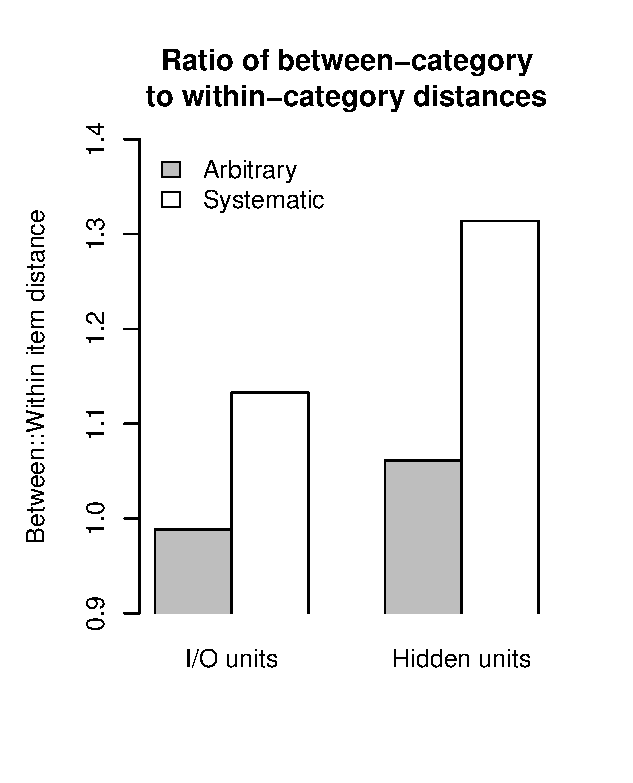
\includegraphics[width=0.5\textwidth]{figures/figure3.eps}
\caption{\label{fig.between_within_dist} Left: Ratio of between-domain to within-domain Euclidean distances for the representations coded over different sets of units in the network, averaged over the 10 model subjects. Distributed representations that encode the domain structure should have large distances for items from different domains and small distances for items from the same domain, and so should show a large ratio. While the systematic I/O units clearly code the domain structure to some degree, the systematic hidden units express the structure more strongly. 
%Right: Mean activation of each unit in the model for domain A items (top) or domain B items (bottom). Though SH units jointly provide better information about item domain, no domain information is apparent in the mean activation of individual units across model subjects. The systematic I/O units, though jointly providing a weaker representation of domain structure, individually show reliable differences in mean activation across model subjects for items from different domains.
}
\end{figure}

With this general understanding of the model behavior, let's consider how it makes explicit the four challenges for brain imaging noted earlier. First, although the SH units jointly encode the same representational structure across model subjects, the contribution of a given hidden unit to this structure varies arbitrarily across model subjects (challenge 1). Second, the mean activations of SH units do not systematically differ for items in the A and B domains: to find the important structure, one must consider the pattern evoked over multiple units (challenge 2). Third, the functional architecture of the model shown in Figure 2 can be anatomically arranged in many different ways (challenge 3). To make this issue explicit, we consider two different topographic arrangements of the functional model. In the first, units within the same layer are always situated as anatomical neighbors, so that the representations encoded by the SH and the AH layers are {\em anatomically localized}. In the second arrangement, we assume that the SH units are {\em spatially intermingled} with the AH units, in a different way across model individuals, so that the representations they encode are {\em anatomically dispersed}. In the results we will consider how well each method identifies the SH units as a function of whether they are localized or dispersed. Finally, the model captures the idea that the units of interest constitute only a small proportion of all the units measured (challenge 4). In the model itself, most of the units encode information irrelevant to the stimulus domain (the 43 arbitrary units plus 22 irrelevant units). The next largest set are the 36 systematic I/O units that encode the domain structure weakly but consistently across subjects. The units of greatest interest, the 7 SH units, constitute just 6\% of all the units in the data. 

\subsection{Summary} 

Though very simple, this auto-encoder network captures each of the challenges noted in the introduction: it acquires distributed internal representations that express representational structure of interest; the way the structure is coded across units varies in different individual models; the structure cannot be discerned from the activations of single units but arises in patterns over multiple units; the relationship between the functional architecture and the underlying model topography can be opaque; and the units that encode the structure we wish to discover are buried in a large number of other measurements. The question we now address is how well different analysis methods fare at discovering representational structure across both systematic I/O units and the SH units, when they are applied to data generated from a sample of model training runs.

